

%\section*{Abstract}
\section*{\textbf{\underline{Abstract}}}

Spatial biases are an intrinsic feature of occurrence data used in species distribution models (SDM). Thinning species occurrences, where records close in the geographic or environmental space are removed from the modeling procedure, is an approach often used to address these biases. However, thinning occurrence data can also negatively affect SDM performance given that the benefits of removing spatial biases might be outweighted by the detrimental effects of data loss caused by this approach. We used real and virtual species to evaluate how spatial and environmental thinning affected different performance metrics of four SDM methods. Virtual species had their occurrence data sampled randomly, evenly-spaced and clustered in the geographic space to simulate different types of spatial biases and several spatial and environmental thinning distances were used to thin the occurrence data. Null datatsets were also generated for each thinning distance where we randomly removed the same number of occurrences that was removed by a thinning distance and compared the results of the thinned and null datasets. We found that spatially or environmentally thinning occurrence data is no better than randomly removing them given that thinned datasets performed similarly to null datasets. Specifically, spatial and environmental thinning led to a general decrease in model performances across all SDM methods. These results were observed for real and virtual species, were positively associated with thinning distance, and were consistent across the different types of spatial biases. Our results suggest that thinning occurrence data usually fails to improve SDM performance and that the use of thinning approaches when modeling species distributions should be carefully considered. 






%-----------------------
\section*{\textbf{\underline{Introduction}}}
%\textbf{\underline{Introduction}}

A species geographic distribution expresses its ecology and evolutionary history \parencite{brown1995, gaston2003} where abiotic conditions, biotic factors, and dispersal ability determine the areas a species can occupy \parencite{soberon2005}. Having a refined knowledge on species distributions is essential as it is a key variable for assessing biogeographical and macroecological patterns \parencite{hortal2015, herkt2017} and to describe the conservation status and extinction risk of a species \parencite{cardillo2008, lee2011}. However, currently there is an incomplete knowledge on the distribution of several species, a shortcoming called the \textit{Wallacean shortfall} \parencite{lomolino2004, whittaker2005, hortal2015}. The ongoing development of species occurrence databases and species distribution models (SDM) have improved the ability to estimate species geographic ranges, partially addressing this Wallacean shortfall \parencite{peterson2011,jetz2012,terribile2018}. Nevertheless, using SDMs to estimate species geographic distribution might be challenging as several factors, such as quality of the data available, affect the performance and predictive ability of these models \parencite{santini2020}.


\paragraph*{}
The Wallacean shortfall is partially driven by spatial biases present during the sampling process such as sampling locations based on proximity to universities and local accessibility \parencite{moerman2006,vale2012,sousa2014,oliveira2016}. This leads species occurrence points (i.e., localities where the species was recorded) to be sampled in a non-random subset of areas from which the species could occupy. Consequently, sampled occurrence points tend to be spatially clustered, a problem that is often observed in online databases \parencite{beck2014, inman2021}. These clustered points has the potential to disproportionately represent the environmental conditions of the most sampled regions rather than representing the set of suitable environmental conditions for a species \parencite{kadmon2004, anderson2011}, which can affect SDM performance \parencite{veloz2009,beck2014}. This occurs because the occurrence points used for training and testing the SDMs might be spatially adjacent, which can lead to higher (inflated) model performances than expected \parencite{bahn2013,radosavljevic2014}. 
 


\paragraph*{}
Although spatial block validation can be used to obtain non-inflated SDM performances \parencite{bahn2013,radosavljevic2014, roberts2017}, it does not remove the bias present in species occurrence data. Background manipulation methods can also be used to address bias in occurrence data, but this approach requires knowledge on the sampling effort for a species, which is rarely available, or a large observation dataset to estimate the biased sampling effort \parencite{phillips2009, ranc2017, inman2021}. Alternatively, thinning approaches are perhaps the most commonly used methods that have been developed to remove spatial biases found in occurrence data \parencite{hidalgo2004,veloz2009,anderson2010,varela2014,aiello2015}. Occurrence points can be thinned based on the geographical \parencite{veloz2009,aiello2015} or environmental \parencite{varela2014} distances between them such that only the most spatially or environmentally unique occurrences are kept and used in the modeling process. The effects of spatial thinning on model performance is unclear \parencite{boria2014, beck2014, varela2014, castellanos2019} and dependent on the ecological characteristic of the species \parencite{steen2021,baker2022}. For example, spatial thinning might not be appropriate for species that have spatially clustered occurrences because it can lead to an undesirable loss of data that negatively affects model performance \parencite{varela2014}. Consequently, environmental thinning has been suggested to be a superior alternative in these situations given that occurrence points are filtered in the environmental space in this approach, which can reduce the data loss experienced by species with spatially clustered occurrences \parencite{varela2014, castellanos2019}. However, regardless of the type of thinning that is used, a challenge during the thinning process is choosing the distance to filter the dataset \parencite{castellanos2019} as using larger thinning distances will inherently remove more occurrence points from the initial dataset. Given that the number of occurrence points has a larger impact on model performance than spatial bias \parencite{gaul2020}, the potential benefits of thinning might be lost if considerably fewer occurrence points are left for the modeling procedure \parencite{steen2021}.




 

\paragraph*{}
Here we examine the effects of spatial and environmental thinning occurrence points on SDM performance for real and virtual species (Figure \ref{fig:concep_sdmthin}). For virtual species, we simulated species that had occurrence data sampled randomly, clustered and evenly-spaced (i.e., a similar distance between the sampled occurrences) in the geographic space. Our goal was to evaluate whether the effectiveness of thinning is dependent on the types of spatial bias observed in occurrence points. We thinned occurrence points considering different thinning distances and used four modeling methods to model the species distributions and four performance metrics to evaluate the models. We compared the results of these models to null models where we randomly removed species occurrence points from the modeling procedure. Spatial and environmental thinning decreased model performance for real and virtual species, and performed no better than null models, suggesting that thinning approaches have limited benefits for SDMs.
%Overall, we found that spatial and environmental thinning presence points decreased model performance for real and virtual species. Moreover, thinned models performed no better than null models, suggesting that thinning approaches have limited benefits for SDMs.

%-----------------------
\section*{\textbf{\underline{Methods}}}
%\section*{Methods}


\paragraph*{Simulating landscapes}\mbox{}\\ 
We simulated 500 landscapes where 500 virtual species would occur. The virtual landscapes were modelled as a raster with 90 X 180 cells where two gradients, one horizontal and another vertical, shaped the species virtual environment (Figure \ref{fig:concep_sdmthin}). The gradients were modelled following a Gaussian distribution \parencite{dallas2020} where the environmental values present in the landscape ranged from 0 to 2.5. A gaussian random field was added into the modelled landscapes in order to simulate a more realistic spatially autocorrelated environment. We randomly selected the strength of the Gaussian random field (ranging from 0.1 to 1.5) to make each virtual landscape a unique set of environmental conditions for a species. The strength of the Gaussian random field added to the landscapes is positively related to how heterogenous the environmental conditions are in the landscape (Appendix A: Figure \ref{fig:S1}). The maximum strength of 1.5 in the Gaussian random field was chosen because at this level the landscape is highly heterogenous but it still maintains its spatially autocorrelated nature (see Appendix A for further information).

%What is the step size again?
%All landscapes were modelled with the value of step size set as 5. 

\paragraph*{Simulating species distributions}\mbox{}\\ 
Species environmental niches, and distributions within these virtual landscapes, were simulated with the \texttt{virtualspecies} R package \parencite{leroy2016}. Species niches were modelled following a Gaussian response to the virtual environment as it has been shown that many species exhibit this response to environmental and ecological gradientes \parencite{oksanen2002, boucher2014} and it is an assumption that studies using virtual species usually adopt \parencite{varela2014,van2016}. The optimum environmental value for each species was randomly chosen and it varied from 1 to 2.2 in each environmental layer with a standard deviation around it ranging from 0.05 to 0.6. We chose this wide range of optimum values (1-2.2) for the two environmental gradients because our goal was to simulate species that are ecologically different regarding the required conditions for their occurrance. Thus, these optimum values allowed us to simulate species that are capable of occupying all the parts of our virtual landscape. The standard deviation around the optimum value was chosen to range between 0.05 and 0.6 because this allowed us to simulate specialist and generalist species when small or large standard deviations were selected respectively. We selected the maximum standard deviation of 0.6 because values above that would make the species unrealistically generalist where it would be able to occupy nearly the entire landscape. A logistic transformation of the species environmental suitability defined the chance of a species occurrence being sampled in a particular cell of the landscape. 


We randomly sampled between 6 to 640 occurrence points to model the distribution of each virtual species. This covers a realistic range of sample sizes that are commonly found when modeling species distributions as rare species often have few sampled occurrence points whereas other species might be better sampled and have more occurrence points available for modeling. We chose a maximum of 640 sampled occurrence points because models perform well with this sample size and performance would likely remain the same if larger sample sizes were used. Three sets of occurrence points were obtained for each species following three types of spatial biases (i.e., random, clustered and evenly-spaced). 

\paragraph*{Clustering and dispersion of sampled occurrences}\mbox{}\\ 
First, we simulated an instance where species occurrence points are sampled randomly across the geographic space. In this case there is no intrinsic sampling bias driving the sampling process. In the second case, we simulated a situation where there is spatial bias in the sampling of occurrence points, and the occurrence points sampled are spatially clustered in the geographic space. Such situation might occur when accessible locations are sampled more often \parencite{botts2011, mair2016}. To simulate this situation, we first randomly selected five initial points that represented five different clusters of occurrence data sampled. Next, we used the distm function from the \texttt{geosphere} package \parencite{hijmans2019} and calculated the distance between the initial points and all other occurrence points. The 50 closest points to each cluster were selected and a point was sampled from it, with closer points having greater probabilities of being sampled. This process was repeated for each cluster of occurrence points until we reached the desired number of occurrences for each species. In the last case, we simulated a case where the sampled points are evenly-spaced from each other. To achieve this goal, we created a grid that covered the entire landscape where the number of cells in the grid would be equal to the number of occurrences desired to be sampled. Occurrence points were sampled from this grid such that points that were closer to the centroid of each cell in the grid had a greater probability of being sampled. All of the data manipulation in this step was done using the \texttt{sf} package \parencite{pabesma2018}. 


\paragraph*{Empirical species distributions}\mbox{}\\ 
To model the distribution of real species we sampled 500 mammal species from the Global Biodiversity Information Facility (GBIF) using the \texttt{rgbif} package \parencite{chamberlain2021}. We removed 61 species that had less than 5 sampled occurrence points from the modeling procedure because it is challenging to realiably model the distribution of such species. We obtained the 19 bioclimatic variables available in the BioClim database \parencite{hijmans2005} to model the species distribution. These variables represent different facets of temperature and precipitation patterns that have been recorded from weather stations across the globe between 1960 and 1990 \parencite{hijmans2005}. The bioclimatic variables were obtained at a resolution of 10 arc-minutes (i.e., $\approx$ 18 km$^2$) covering the Americas. A Principal Component Analysis (PCA) was performed on these variables and the first two axes explained 80\% of the variance of the data and were used to model the species distribution.


\paragraph*{Spatial and environmental thinning}\mbox{}\\ 
Spatial thinning for real species was done using the thin function from the \texttt{spThin} package \parencite{aiello2015}. In this function a pair-wise distance matrix between all occurrence points is calculated based on a chosen distance and a neighbor point of the observation with the most neighbours is removed. This process is repeated until there are no more points with neighbors based on the chosen distance. For each species, we thinned occurrence points with a distance of 16, 32, 64 and 128 km. These values were chosen because our environmental values were obtained at the spatial resolution of ~16 km$^2$. For the virtual species we spatially thinned the occurrence points following a similar framework. Virtual species only have one occurrence point per cell (i.e., the centroid of the cell). We used the select.window function from the \texttt{CommEcol} package \parencite{melo2019} and removed neighbour points to the focal occurrence points based on a chosen distance. We chose the distances of 2,4,8 and 16. In the distance of two, all eight neighbor cells to a focal point are selected and their points are removed. Similarly, with a distance of 4, 16 of neighbor cells are selected and their points are removed; with a distance of 8, 32 neighbor cells are selected and their points are removed; with a distance of 16, 64 neighbor cells are selected and their points are removed. Thus, thinning distance doubles for every increase in the distance used for virtual species, which is analogous to how we thinned the occurrence points of real species.

Environmental thinning virtual and real species occurrence points was done using the method developed by \textcite{varela2014}. In this framework, bins are created based on a chosen environmental distance and then only one point that falls within an environmental bin is selected for the modeling. Thus, more points are discarded when larger environmental distances are used. For real species, environmental thinning was based on the two PCA axes used to model their distribution, while for virtual species it was based on the two virtual climatic conditions. The environmental intervals we used for both real and virtual species were 0.05, 0.1, 0.2 and 0.4. We used the envSample function to environmentally thin our data \parencite{varela2014}. 

\paragraph*{Comparing thinned and null models}\mbox{}\\ 
Since thinning occurrence points decreases the number of points available to model the species distribution and that this alone can negatively affect SDM performance \parencite{loiselle2008,tessarolo2014}, we also generated null datasets for all spatial and environmental thinning distances we used. In the null dataset, we randomly removed the same number of occurrence points that were removed by a specific spatial or environmental thinning distance for a species. Thus, a similar performance between thinned and null datasets would suggest that the benefits of removing spatial bias through thinning approaches are countered by the loss of occurrence points that are important to model the species distribution.

%%Putting [h!]
\paragraph*{Modeling species distributions}\mbox{}\\ 
We evaluated the effects that spatial and environmental thinning have on the performance of MaxEnt, support vector machine (SVM), generalized linear models (GLM) and generalized additive models (GAM) modeling methods. We chose these modeling methods because they are commonly used methods that utilize presence/pseudo-absence data. Specifically, MaxEnt is a widely used machine learning method that generally performs well \parencite{elith2010,santini2020}. SVM is also a machine learning method that performs well for species with limited occurrence data \parencite{scholkopf2001, tax2004, drake2006}. GLM is a simple regression-based modeling method \parencite{nelder1972, loyola2012} and GAM is an extension of GLM that allows some predictors to be modelled non-parametrically \parencite{guisan2002}. MaxEnt models were run with the maxent function from the R \texttt{dismo} package \parencite{hijmans2017}; SVM models were run with the svm function from the R \texttt{kernlab} package \parencite{karatzoglou2019}; GLM models were run using the glm function from the R \texttt{stats} package \parencite{R}; and GAM models were run using the gam function from the R \texttt{mgcv} package \parencite{wood2017}.

As class imbalances in the number of occurrence/pseudo-absence points can affect model inter-comparisons \parencite{mcpherson2004, liu2005}, we kept prevalence at 0.5, where 50\% of the data are occurrences and 50\% are pseudo-absences \parencite{senay2013, iturbide2015}. Pseudo-absences were randomly sampled for virtual and real species, sampling from a 200km circular buffer for real species and from the entire landscape for virtual species. Next, we applied a cross-validation procedure where we randomly split our occurrence data into two datasets: 75\% of the data were used to train the models and the other 25\% of the data were used to test the models, repeating the sampling process 20 times. Since we only have one dataset for the real species, we used that same dataset in each of the 20 sampling process. For the virtual species, we have 20 unique dataset, where the number of occurrences and pseudo-absences was the same in each dataset, but different occurrences and pseudo-absences were sampled in each dataset. Similar patterns of model performance were observed for virtual species when the same and unique datasets were used to model the species distribution in each sampling process (Appendix A: Figure \ref{fig:S2}). Thus, using the same and unique datasets during the cross-validation procedure does not affect the estimation of the virtual species distributions. Virtual species SDMs were evaluated with independent data (i.e., data that were not sampled to model the species distributions).

\paragraph*{Assessing model performance}\mbox{}\\ 
We evaluated SDM performance with regards to accuracy, calibration, discrimination power (hereafter discrimination) and precision \parencite{norberg2019}. Accuracy measures the agreement between the model predicted values and the observed values (i.e., how close the predicted values are to the observed values). We measured accuracy as the absolute difference between the predicted (varying from 0 to 1) and the observed (0 for pseudo-absence and 1 for occurrence) values. Calibration was assessed as the statistical accuracy between the predicted and observed values. As a measure of calibration, we calculated the root-mean-square error (RMSE) between the predicted and observed values in 10 probability bins (see methods section in Appendix A and Appendix A: Figure \ref{fig:rmse} for details). Discrimination evaluates how well the predictive values of a model can differ between occurrences and pseudo-absences. We used the area under the receiver operating characteristic curve (AUC) \parencite{fielding1997} to evaluate discrimination. At last, precision measures the breadth of the predictive distribution of the models. As a measure of precision we calculated the square root of the product of the probability of species occurrence in a cell times the probability of the species absence in that same cell. All the performance metrics were averaged across species. To facilitate the interpretation of the results, we reversed the signs of the performance metrics when applicable, such that higher performance values always indicated a higher discrimination, calibration, accuracy or precision of the models.

We used a linear mixed-effect (LMM) model to evaluate whether thinning occurrence points affected SDM performances. In this framework, model performance was used as the response variable and spatial and environmental thinning distances were used as fixed effects and species was used as a random effect. The non-filtered dataset was used as the baseline case to evaluate the effects of thinning occurrence points on model performance. We present the effects of thinning on MaxEnt discrimination power (AUC) in the results section except where noted otherwise.



%-----------------------
\section*{\textbf{\underline{Results}}}
%\section*{Results}

\paragraph*{General effects of thinning occurrence points}\mbox{}\\ 
Thinning occurrence points consistently decreased model performance irrespective of spatial bias for real and virtual species (Figure \ref{fig:Figure2}, Table \ref{tab:LMMtable}). Using larger spatial and environmental thinning distances resulted in fewer occurrence points being available for modeling (Appendix A: Figure \ref{fig:S3}) and worse model performances were observed in these cases. Spatially and environmentally thinning species occurrence points was functionally the same as removing occurrences randomly given that model performances were similar between thinned and null datasets (i.e., error bars overlapping zero, Figure \ref{fig:Figure3}).




\paragraph*{Thinning real and virtual species occurrences}\mbox{}\\ 
Spatial thinning had stronger negative effects on clustered occurrences relative to random or evenly-spaced occurrences (Figure \ref{fig:Figure2}). Specifically, even the smallest spatial distances caused significant decreases in model performance of real and virtual species with clustered occurrences (Table \ref{tab:LMMtable}). Alternatively, virtual species with random and evenly-spaced occurrences only experienced significant decreases in model performance when the two largest spatial distances were used (Table \ref{tab:LMMtable}), suggesting that these species are less susceptible to the negative effects of spatial thinning. 

Environmental thinning decreased model performance similarly across real and all virtual species (Figure \ref{fig:Figure2}). In general, environmentally thinning occurrence points using the smallest environmental distance did not affect model performance, but model performance quickly deteriorated for all species as the environmental distance used increased (Table \ref{tab:LMMtable}). Thus, environmental thinning had more consistent negative effects on SDM performance than spatial thinning. 








\paragraph*{Effects of thinning on different performance metrics and modeling methods }\mbox{}\\ 
In general, discrimination, accuracy, calibration, and precision were positively correlated to each other (Figure \ref{fig:Figure4}), suggesting a general agreement between the performance metrics we used to evaluate the SDMs. As with discrimination, thinning occurrence points also decreased models accuracy (Appendix A: Figure \ref{fig:S4}), precision (Appendix A: Figure \ref{fig:S5}), and calibration (Appendix A: Figure \ref{fig:S6}), indicating that models are in general making more incorrect predictions when occurrence points are thinned.


Overall, GLM tended to have the worst performance across the modeling methods whereas GAM, SVM and MaxEnt had superior performances (see Appendix A). Although thinning had consistent negative effects on the performance of the four modeling methods we assessed, some methods were more affected by thinning than others. For example, SVM (Appendix A: Figures \ref{fig:S7}-\ref{fig:S10}) and GLM (Appendix A: Figures \ref{fig:S11}-\ref{fig:S14}) had relatively similar model performances for the virtual species when the non-thinned and thinned datasets were used. On the other hand, MaxEnt (Figure \ref{fig:Figure2}, Appendix A: Figures \ref{fig:S4}-\ref{fig:S6}) and GAM (Appendix A: Figures \ref{fig:S15}-\ref{fig:S18}) had more significant decreases in model performance when occurrences were thinned. This result suggests that number of occurrence points is more important to efficiently model species distributions for some modeling methods (i.e., MaxEnt and GAM) than for others (i.e., SVM and GLM). The only improvement in model performance caused by thinning was observed when precision was the performance metric for GLM (Appendix A: Figure \ref{fig:S13}) and GAM (Appendix A: Figure \ref{fig:S17}). The fact that improvement in model performance was not observed by any other performance metric and modeling method we considered shows the general ineffectiveness of thinning approaches to address spatial bias (see Appendix A for details). 


%-----------------------
\section*{\textbf{\underline{Discussion}}}
%\section*{Discussion}

\paragraph*{}
%General bits
In general, we found that spatial and environmental thinning species occurrence points led to a consistent decrease in SDM performance. These reductions in performance were constant across real and virtual species, performance metrics, modeling methods, and were positively associated with thinning distance. Real species and virtual species with clustered points were particularly susceptible to spatial thinning, indicating that this approach might be inadequate for situations where its use is generally suggested \parencite{beck2014, boria2014}. Environmental thinning had similar negative effects on model performance for all species, showing a general limitation of this approach to address biases in occurrence points. Finally, we showed that thinned models perform similarly to null models, suggesting that thinning occurrence points is not better than randomly removing them, further highlighting the inefficacy of thinning approaches in improving model performance. Taken together, our results show that using thinning approaches to remove spatial biases from species occurrence data often negatively affected SDM performance under different modeling scenarios.


\paragraph*{}
%Effects of thinning
Thinning occurrence points before modeling species distributions has the goal of removing sampling bias that is often found in occurrence data \parencite{varela2014, aiello2015}. Although spatial and environmental thinning can improve model performance in individual cases \parencite{boria2014, varela2014}, thinning can have mixed effects on model performance when it is assessed considering several species \parencite{steen2021,inman2021, baker2022}. We expand these results by showing that, when considering a broad ecological context with hundreds of real and virtual species, the effects of spatial and environmental thinning on model performance can often be negative and no different than null expectations. The decrease in model performance caused by spatial thinning is thought to be a consequence of the information loss caused by this approach \parencite{varela2014}. Environmental thinning is also likely leading to a similar degree of information loss given its stronger impacts on virtual species than spatial thinning. This general negative impact of thinning is not unexpected given that number of occurrence points can have a greater impact on model performance than spatial bias \parencite{gaul2020}, which also explains why using larger thinning distances led to worse model performances.






\paragraph*{}
%Different metrics
One of the most commonly used performance metrics to evaluate SDMs is AUC because it is a threshold independent metric \parencite{fourcade2018}. However, relying on a single performance metric when assessing the effects of thinning on SDMs is problematic \parencite{castellanos2019} and using alternative metrics that capture different aspects of model effectiveness under different scenarios allows for a more complete assessment of model performance \parencite{norberg2019, lotterhos2022}. We show that discrimination, accuracy, calibration and precision are generally positively correlated to each other and are generally negatively affected by thinning. Specifically, thinning occurrence points not only decreased the ability of the models to discern different types of values (lower discrimination), but also led models to be more biased (lower accuracy) and less consistent (lower calibration) and precise (lower precision). Although thinning made some models (i.e., GLM and GAM) more precise, they also had lower accuracy, indicating that these models were more confident in making incorrect predictions. Thus, evaluating models considering single performance metrics should be avoided as it can potentially lead to misleading conclusions regarding the effects of thinning on SDMs.



\paragraph*{}
Our results contribute to a growing body of evidence showing that spatially or environmentally thinning occurrence points might not necessarily improve SDM performance \parencite{castellanos2019, steen2021, inman2021}. Nonetheless, we recognize that our study has some limitations such as with regards to the types of spatial biases we simulated in our virtual species. For example, real species usually have occurrence points sampled in a biased manner \parencite{vale2012,sousa2014,oliveira2016} that leads their occurrences points to be mostly spatially clustered \parencite{beck2014, inman2021} while the occurrence of species with random or evenly-spaced occurrence points might be less common. Nevertheless, we show that the effects of thinning were similar across the three different types of spatial bias we considered, indicating that thinning has consistent negative effects on model performance regardless of the type of spatial bias found in the data that is used in SDMs. Additionally, more realistic effects of thinning on SDM performance might be obtained when thinning distances are chosen considering the region, spatial scale and species being studied \parencite{castellanos2019}. Although we did not consider these factors when choosing thinning distances, the fact that we used a wide range of thinning distances and that SDM performance consistently decreased across these different distances suggests that the potential positive effects of thinning on SDM performance are limited.



\paragraph*{}
Evaluating the effects of thinning considering only real species is challenging because there is no knowledge on the "true" distribution of these species, which complicates the assessment of the models, a problem that is overcome with virtual species \parencite{miller2014, moudry2015}. On the other hand, assessing the effects of thinning considering only virtual species might also not be optimal given that these species are usually modelled following simplistic assumptions that might not be observed in the real world, such as the lack of dispersal limitation or interspecific interactions that are important in controlling real species geographic distributions \parencite{soberon2005}. Here, we use a set of real and virtual species to provide strong evidence that thinning occurrence points often decreases SDM performance. Although higher model performance does not necessarily mean more biologically realistic predictions \parencite{godsoe2010,fourcade2018}, the fact that model performance consistently decreased in all circumstances considered in our study, and that these models performed no better than null models, highlights the limitation of thinning approaches to improve SDM performance. These negative effects of thinning might be particularly pronounced when rare species are considered given that modeling their distributions is already a challenging task because of their limited data availability \parencite{steen2021}. Although thinning might not always be detrimental for SDM performance, our results suggest that its use should be considered carefully given that it can easily lead to decreases in model performance.

\section*{\textbf{\underline{Figures}}}

\begin{figure}[H]
\centering
%\graphicspath{ {c:/Teste/Chapter-1-Protocol/Conceptual Figure/} }
%
\includegraphics{Teste}
\centerline{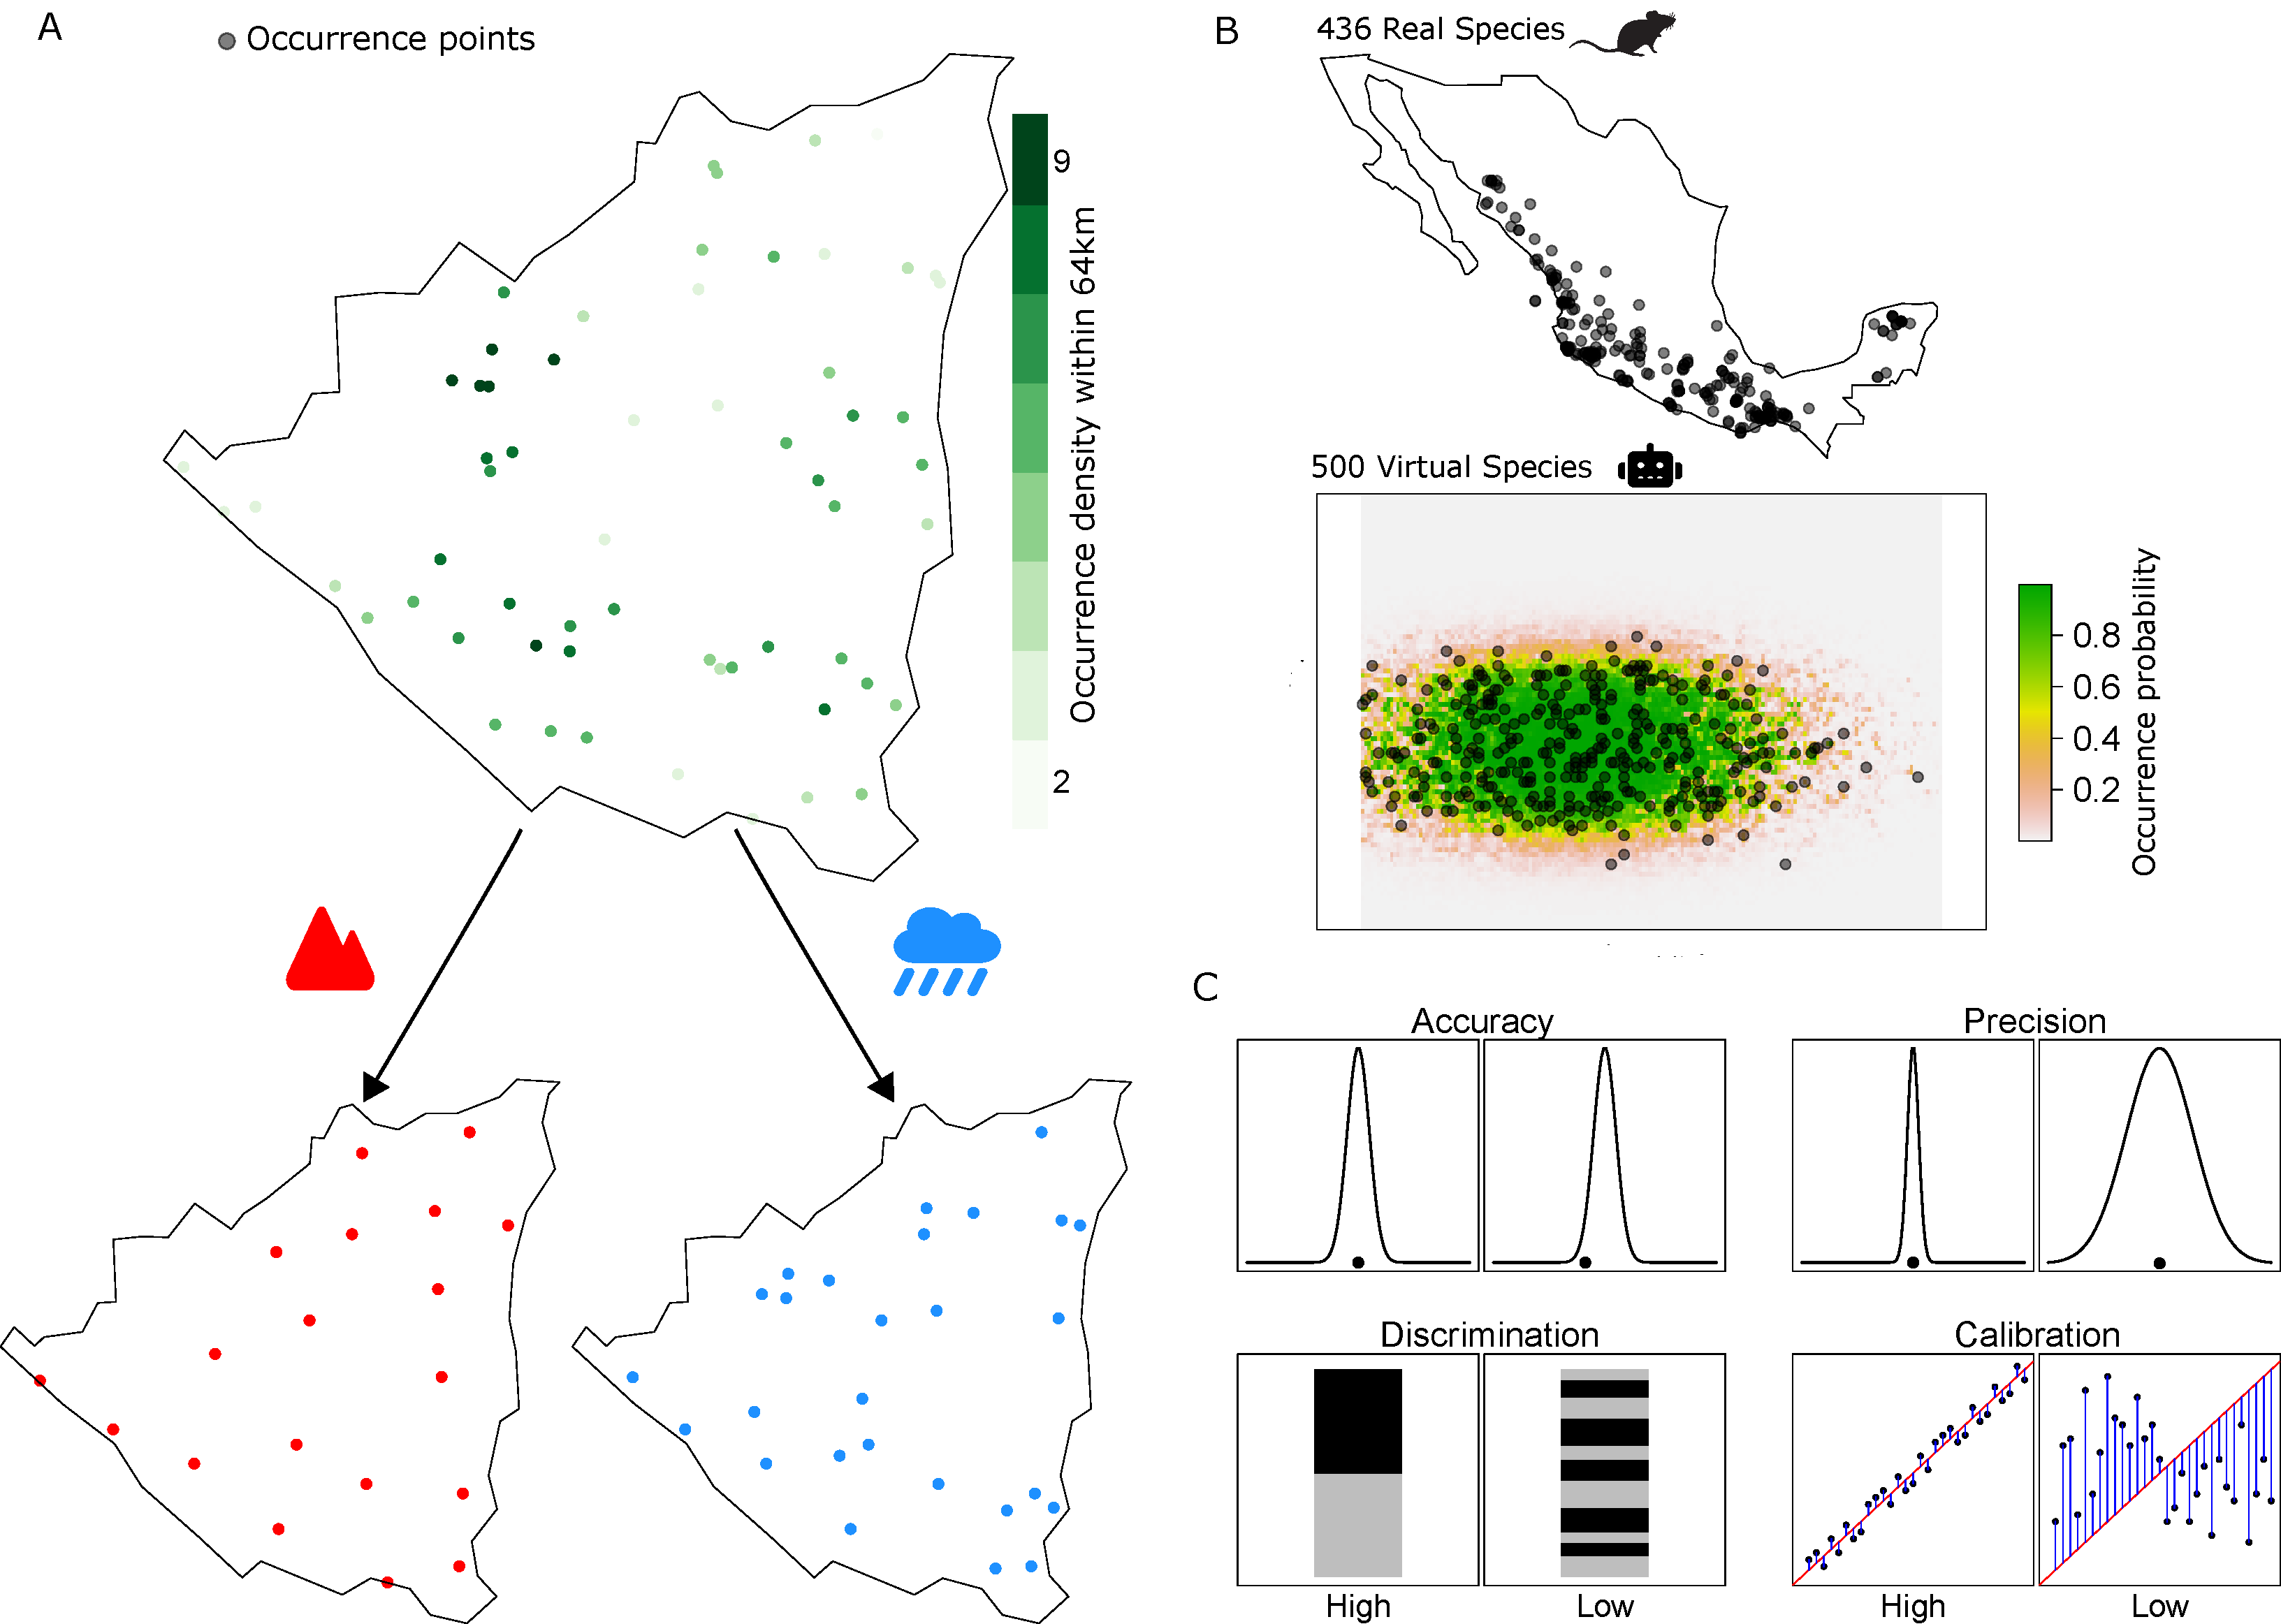
\includegraphics[width=1\textwidth]{Plots/Teste}}
\caption[Thinning occurrence data]{An example of how spatial (red mountain) and environmental (blue cloud) thinning can lead to a selection of different sets of occurrence points that are used to model the species distributions and that could influence model performance measures.}
\label{fig:concep_sdmthin}
\end{figure}
  

\begin{figure}[H]
\centering
%\graphicspath{ {c:/Teste/Chapter-1-Protocol/Manuscript/Plots/} }
\centerline{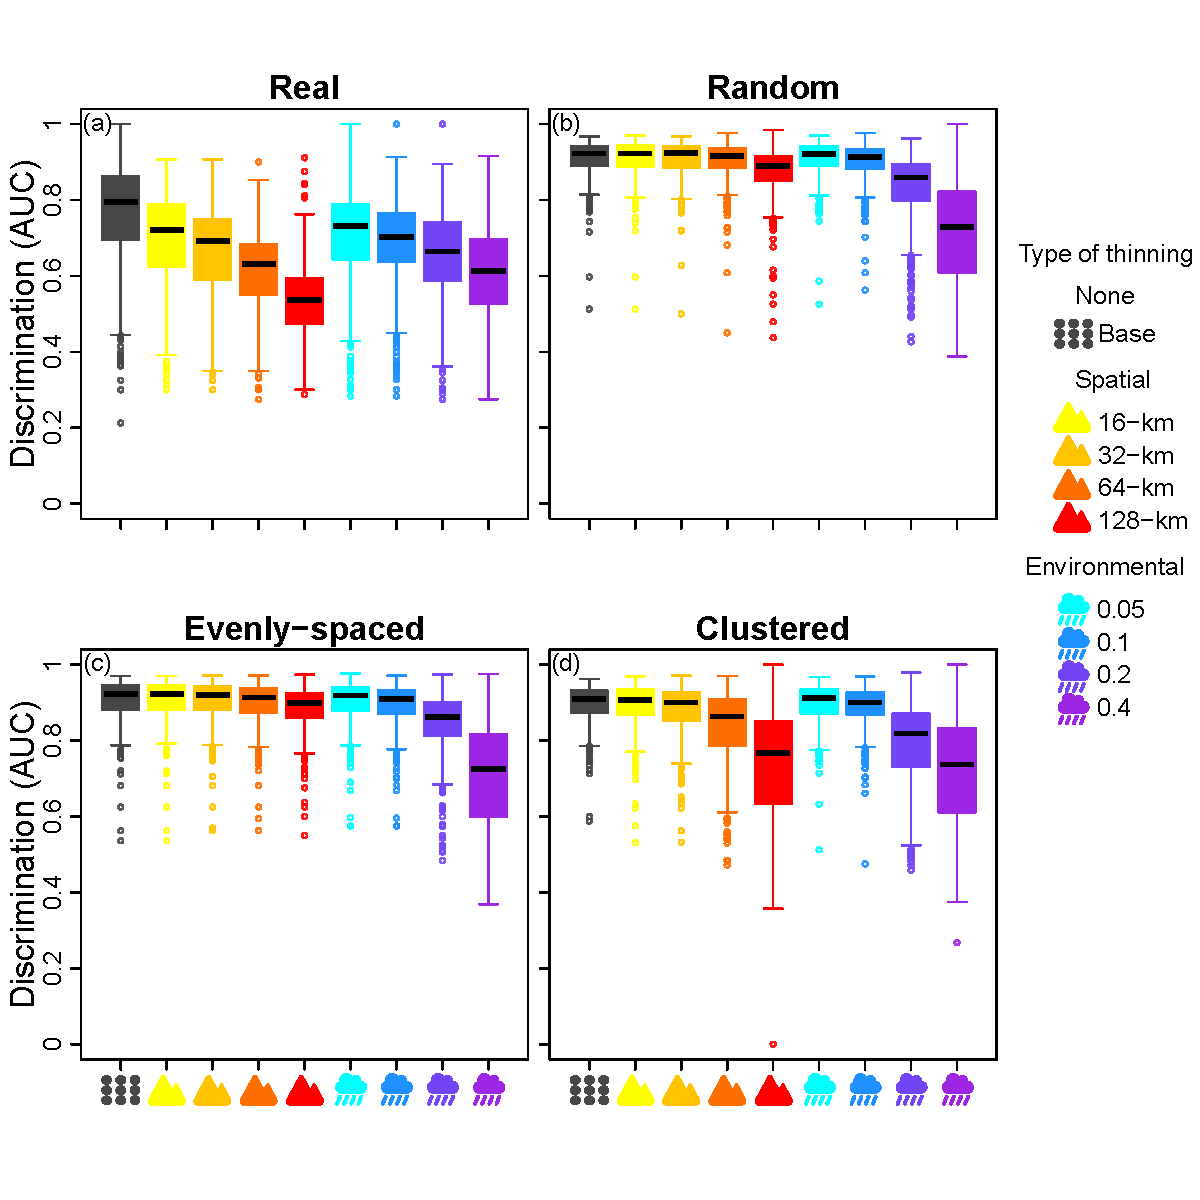
\includegraphics[width=1\textwidth]{Plots/Figure2}}
\caption[Effects of spatial and environmental thinning on model performance]{The effects of spatial and environmental thinning on MaxEnt discrimination (Area Under the Curve, AUC) for real species (a), and virtual species with random (b), evenly-spaced (c), and clustered (d) sampled occurrence points. }
\label{fig:Figure2}
\end{figure}

\begin{figure}[H]
\centering
%\graphicspath{ {c:/Teste/Chapter-1-Protocol/Manuscript/Plots/} }
\centerline{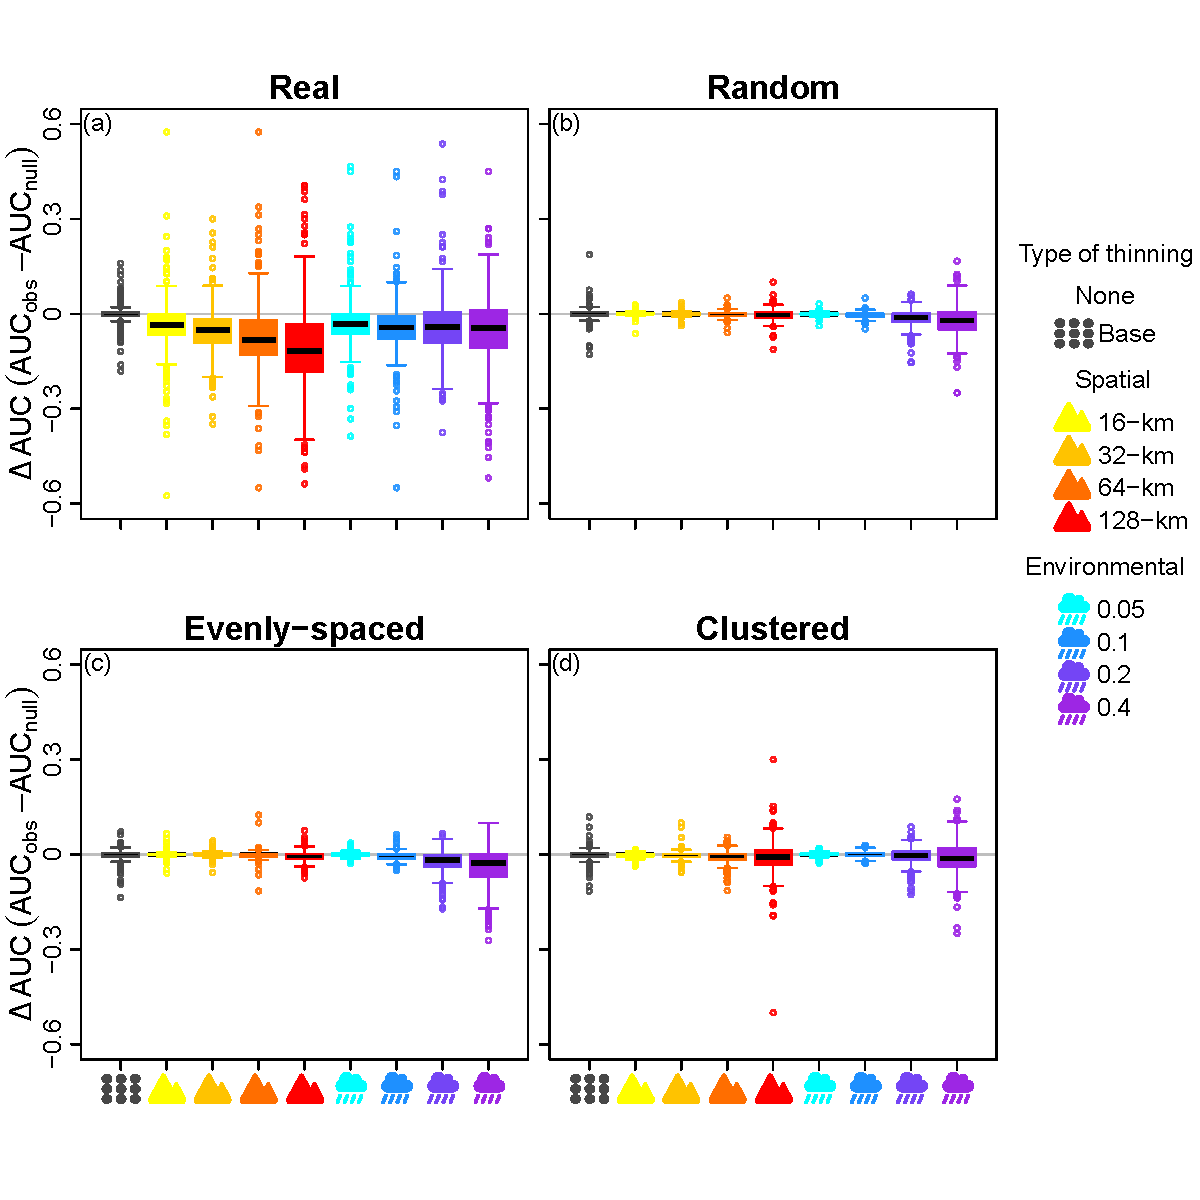
\includegraphics[width=1\textwidth]{Plots/Figure3}}
\caption[Model performance of thinned and null data]{Differences in discrimination (Area Under the Curve (AUC), $\Delta$AUC) of models trained with thinned (AUC$_{obs}$) and null (AUC$_{null}$) data for real species (a), and virtual species with random (b), evenly-spaced (c), and clustered (d) sampled occurrence points.} 
\label{fig:Figure3}
\end{figure}


\begin{figure}[H]
\centering
%\graphicspath{ {c:/Teste/Chapter-1-Protocol/Manuscript/Plots/} }
\centerline{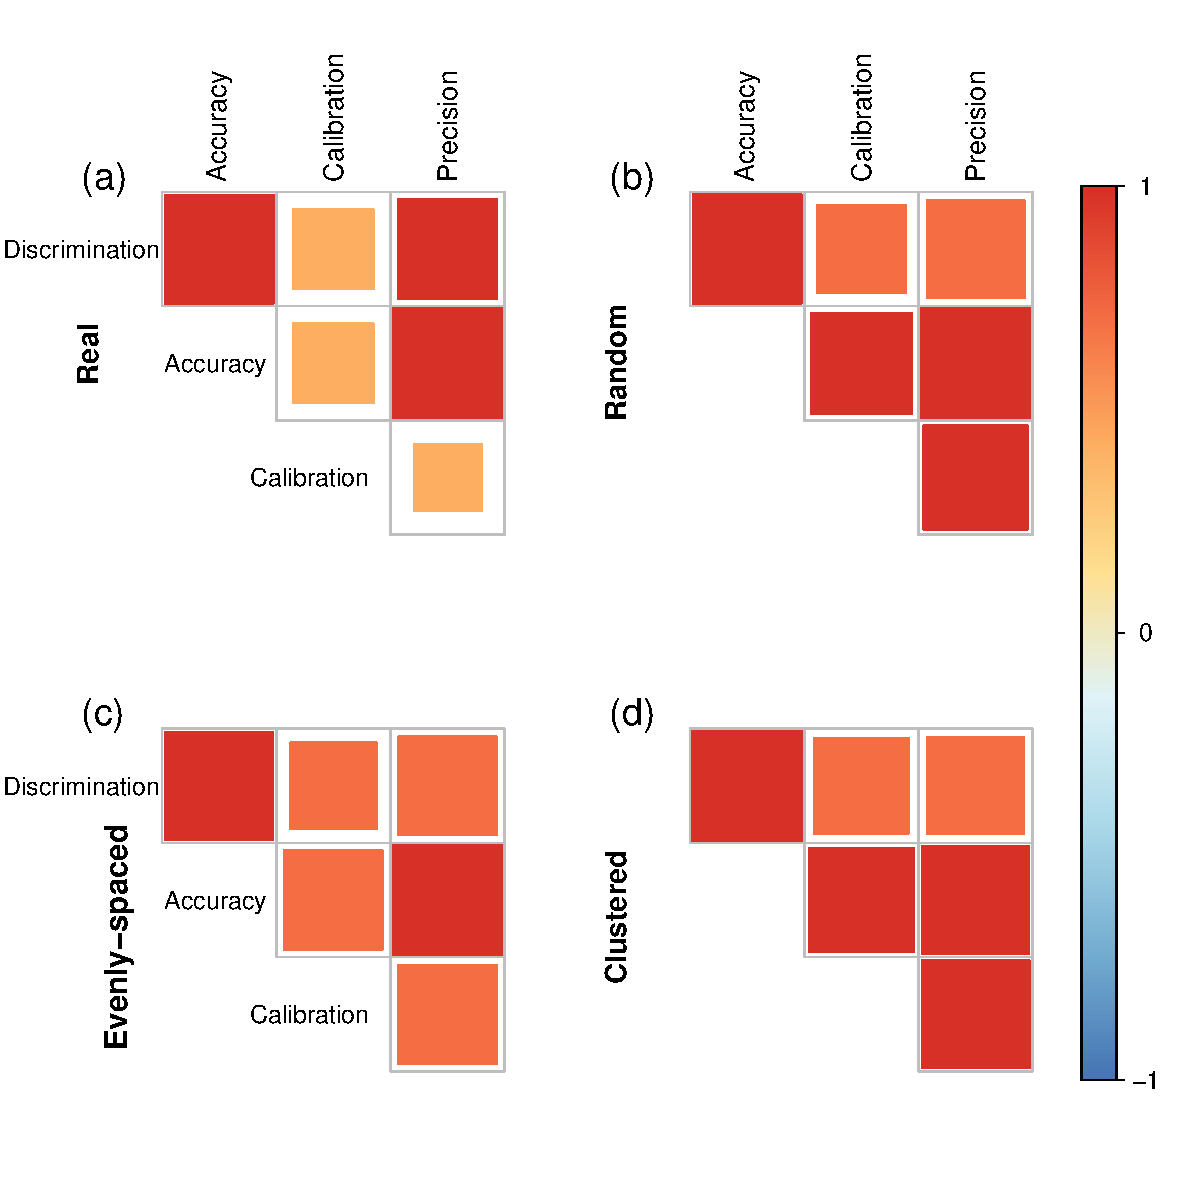
\includegraphics[width=1\textwidth]{Plots/Figure4}}
\caption[Correlation between performance metrics]{Correlation between the performance metrics for real species (a), and virtual species with random (b), evenly-spaced (c), and clustered (d) sampled occurrence points.}
\label{fig:Figure4}
\end{figure}

\section*{\textbf{\underline{Tables}}}
\begin{table}[H]
\centering
\caption[Results from linear mixed effect models]{Fitted linear mixed effects models showing the negative effects of thinning on SDM discrimination (Area Under the Curve, AUC) for real and virtual species with random, evenly-spaced and clustered spatial bias in sampled occurrence points. Significant results ($p$ < 0.05 are highlighted in bold).}
\begin{tabular}{ccccccc}
  \hline
Species & Thinning & Estimate & SE & d.f. & t & p-value \\ 
  \hline
\multirow{8}{*}{\rotatebox{90}{Real}} & S-16 & -0.067 & 0.005 & 3444.2 & -14.464 & \textbf{<0.001} \\ 
   & S-32 & -0.099 & 0.005 & 3444.3 & -21.416 & \textbf{<0.001} \\ 
   & S-64 & -0.152 & 0.005 & 3444.5 & -32.818 & \textbf{<0.001} \\ 
   & S-128 & -0.229 & 0.005 & 3445.0 & -49.289 & \textbf{<0.001} \\ 
   & E-10 & -0.060 & 0.005 & 3443.9 & -12.954 & \textbf{<0.001} \\ 
   & E-15 & -0.076 & 0.005 & 3443.9 & -16.490 & \textbf{<0.001} \\ 
   & E-20 & -0.107 & 0.005 & 3444.3 & -23.269 & \textbf{<0.001} \\ 
   & E-25 & -0.158 & 0.005 & 3444.4 & -34.147 & \textbf{<0.001} \\\hline 
   \multirow{8}{*}{\rotatebox{90}{Random}} & S-16 & -0.000 & 0.003 & 3992.0 & -0.018 & 0.986 \\ 
   & S-32 & -0.001 & 0.003 & 3992.0 & -0.376 & 0.707 \\ 
   & S-64 & -0.008 & 0.003 & 3992.0 & -2.245 & \textbf{0.025}\\ 
   & S-128 & -0.034 & 0.003 & 3992.0 & -10.078 & \textbf{<0.001} \\ 
   & E-10 & -0.002 & 0.003 & 3992.0 & -0.498 & 0.619 \\ 
   & E-15 & -0.009 & 0.003 & 3992.0 & -2.704 & \textbf{0.007}\\ 
   & E-20 & -0.076 & 0.003 & 3992.0 & -22.641 & \textbf{<0.001} \\ 
   & E-25 & -0.196 & 0.003 & 3992.0 & -58.002 & \textbf{<0.001} \\\hline 
   \multirow{8}{*}{\rotatebox{90}{Evenly-spaced}} & S-16 & -0.001 & 0.003 & 3992.0 & -0.174 & 0.862 \\ 
  & S-32 & -0.003 & 0.003 & 3992.0 & -1.012 & 0.312 \\ 
  & S-64 & -0.008 & 0.003 & 3992.0 & -2.683 & \textbf{0.007} \\ 
  & S-128 & -0.021 & 0.003 & 3992.0 & -6.975 & \textbf{<0.001}\\ 
  & E-10 & -0.004 & 0.003 & 3992.0 & -1.296 & 0.195 \\ 
  & E-15 & -0.014 & 0.003 & 3992.0 & -4.697 & \textbf{<0.001} \\ 
  & E-20 & -0.061 & 0.003 & 3992.0 & -20.122 & \textbf{<0.001} \\ 
  & E-25 & -0.197 & 0.003 & 3992.0 & -65.381 & \textbf{<0.001} \\\hline 
   \multirow{8}{*}{\rotatebox{90}{Clustered}} & S-16 & -0.002 & 0.004 & 3992.0 & -0.379 & 0.704 \\ 
   & S-32 & -0.013 & 0.004 & 3992.0 & -3.164 & \textbf{0.002} \\ 
   & S-64 & -0.058 & 0.004 & 3992.0 & -13.672 &\textbf{<0.001}\\ 
   & S-128 & -0.155 & 0.004 & 3992.0 & -36.414 & \textbf{<0.001}\\ 
   & E-10 & 0.003 & 0.004 & 3992.0 & 0.739 & 0.460 \\ 
   & E-15 & -0.006 & 0.004 & 3992.0 & -1.410 & 0.159 \\ 
   & E-20 & -0.101 & 0.004 & 3992.0 & -23.732 & \textbf{<0.001}\\ 
   & E-25 & -0.175 & 0.004 & 3992.0 & -41.116 & \textbf{<0.001}\\ 
   \hline
\end{tabular} 
\label{tab:LMMtable}
\end{table}



















